\begin{frame}{Neutron Reaction Position $K^- d \rightarrow "n_{spec}" \pi^- \Sigma^+_{forward}$}
  \centering
  $\Sigma^+_{forward}$は過去の$K^- p\rightarrow \pi^-\Sigma^+$の角分布をシミュレート
  \begin{tabular}{cc}
    \begin{minipage}{0.6\hsize}
      \begin{figure}
        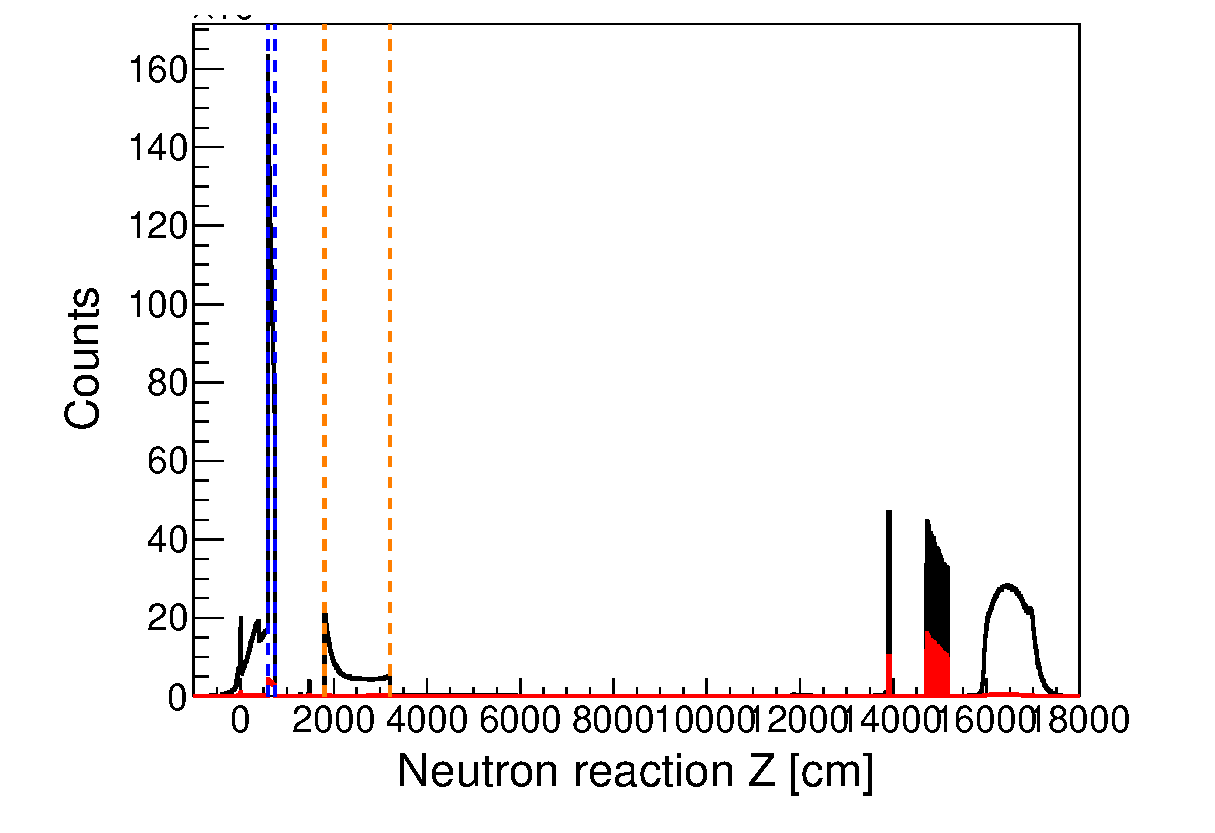
\includegraphics[width=6cm]{../pic/sim/n_reaction_z_pimSp.eps}
      \end{figure}
      \vspace{-4mm}
      \centering
      \scriptsize
      $n_{\Sigma decay}$の反応z位置、\\
      オレンジ破線が牛若,青破線がCDSのエンドキャップ\\
      黒はすべて赤は$n \pi^+ \pi^-$を測定できたもの\\
      15000mm付近のスパイクはNCでの反応\\
    \end{minipage}

    \begin{minipage}{0.4\hsize}
      \begin{figure}
        \includegraphics[width=4cm]{../pic/sim/n_reaction_xy_EndCap_pimSp.eps}
      \end{figure}
      \vspace{-4mm}
      \centering
      \scriptsize
      CDS Endcapでの$n_{forward}$の反応xy位置、\\
      $\pi^+ \pi^- n$の測定は要求していない\\
    \end{minipage}
  \end{tabular}
\end{frame}
